Tunel $ \Tau $ v molekule je v našem případě modelován posloupností koulí o různých poloměrech umístěných v prostoru. Pro posloupnost koulí $ \Tau = \{S_i\}_{i=0}^{n} $ navíc platí $ S_i \bigcap S_{i+1} \neq \emptyset $ pro všechna $ 0 \leq i < n $.
Pro představu jak takový tunel může vypadat uvádíme obrázek \ref{fig:basic_tunnel}.
\begin{figure}[ht]
  	\centering
	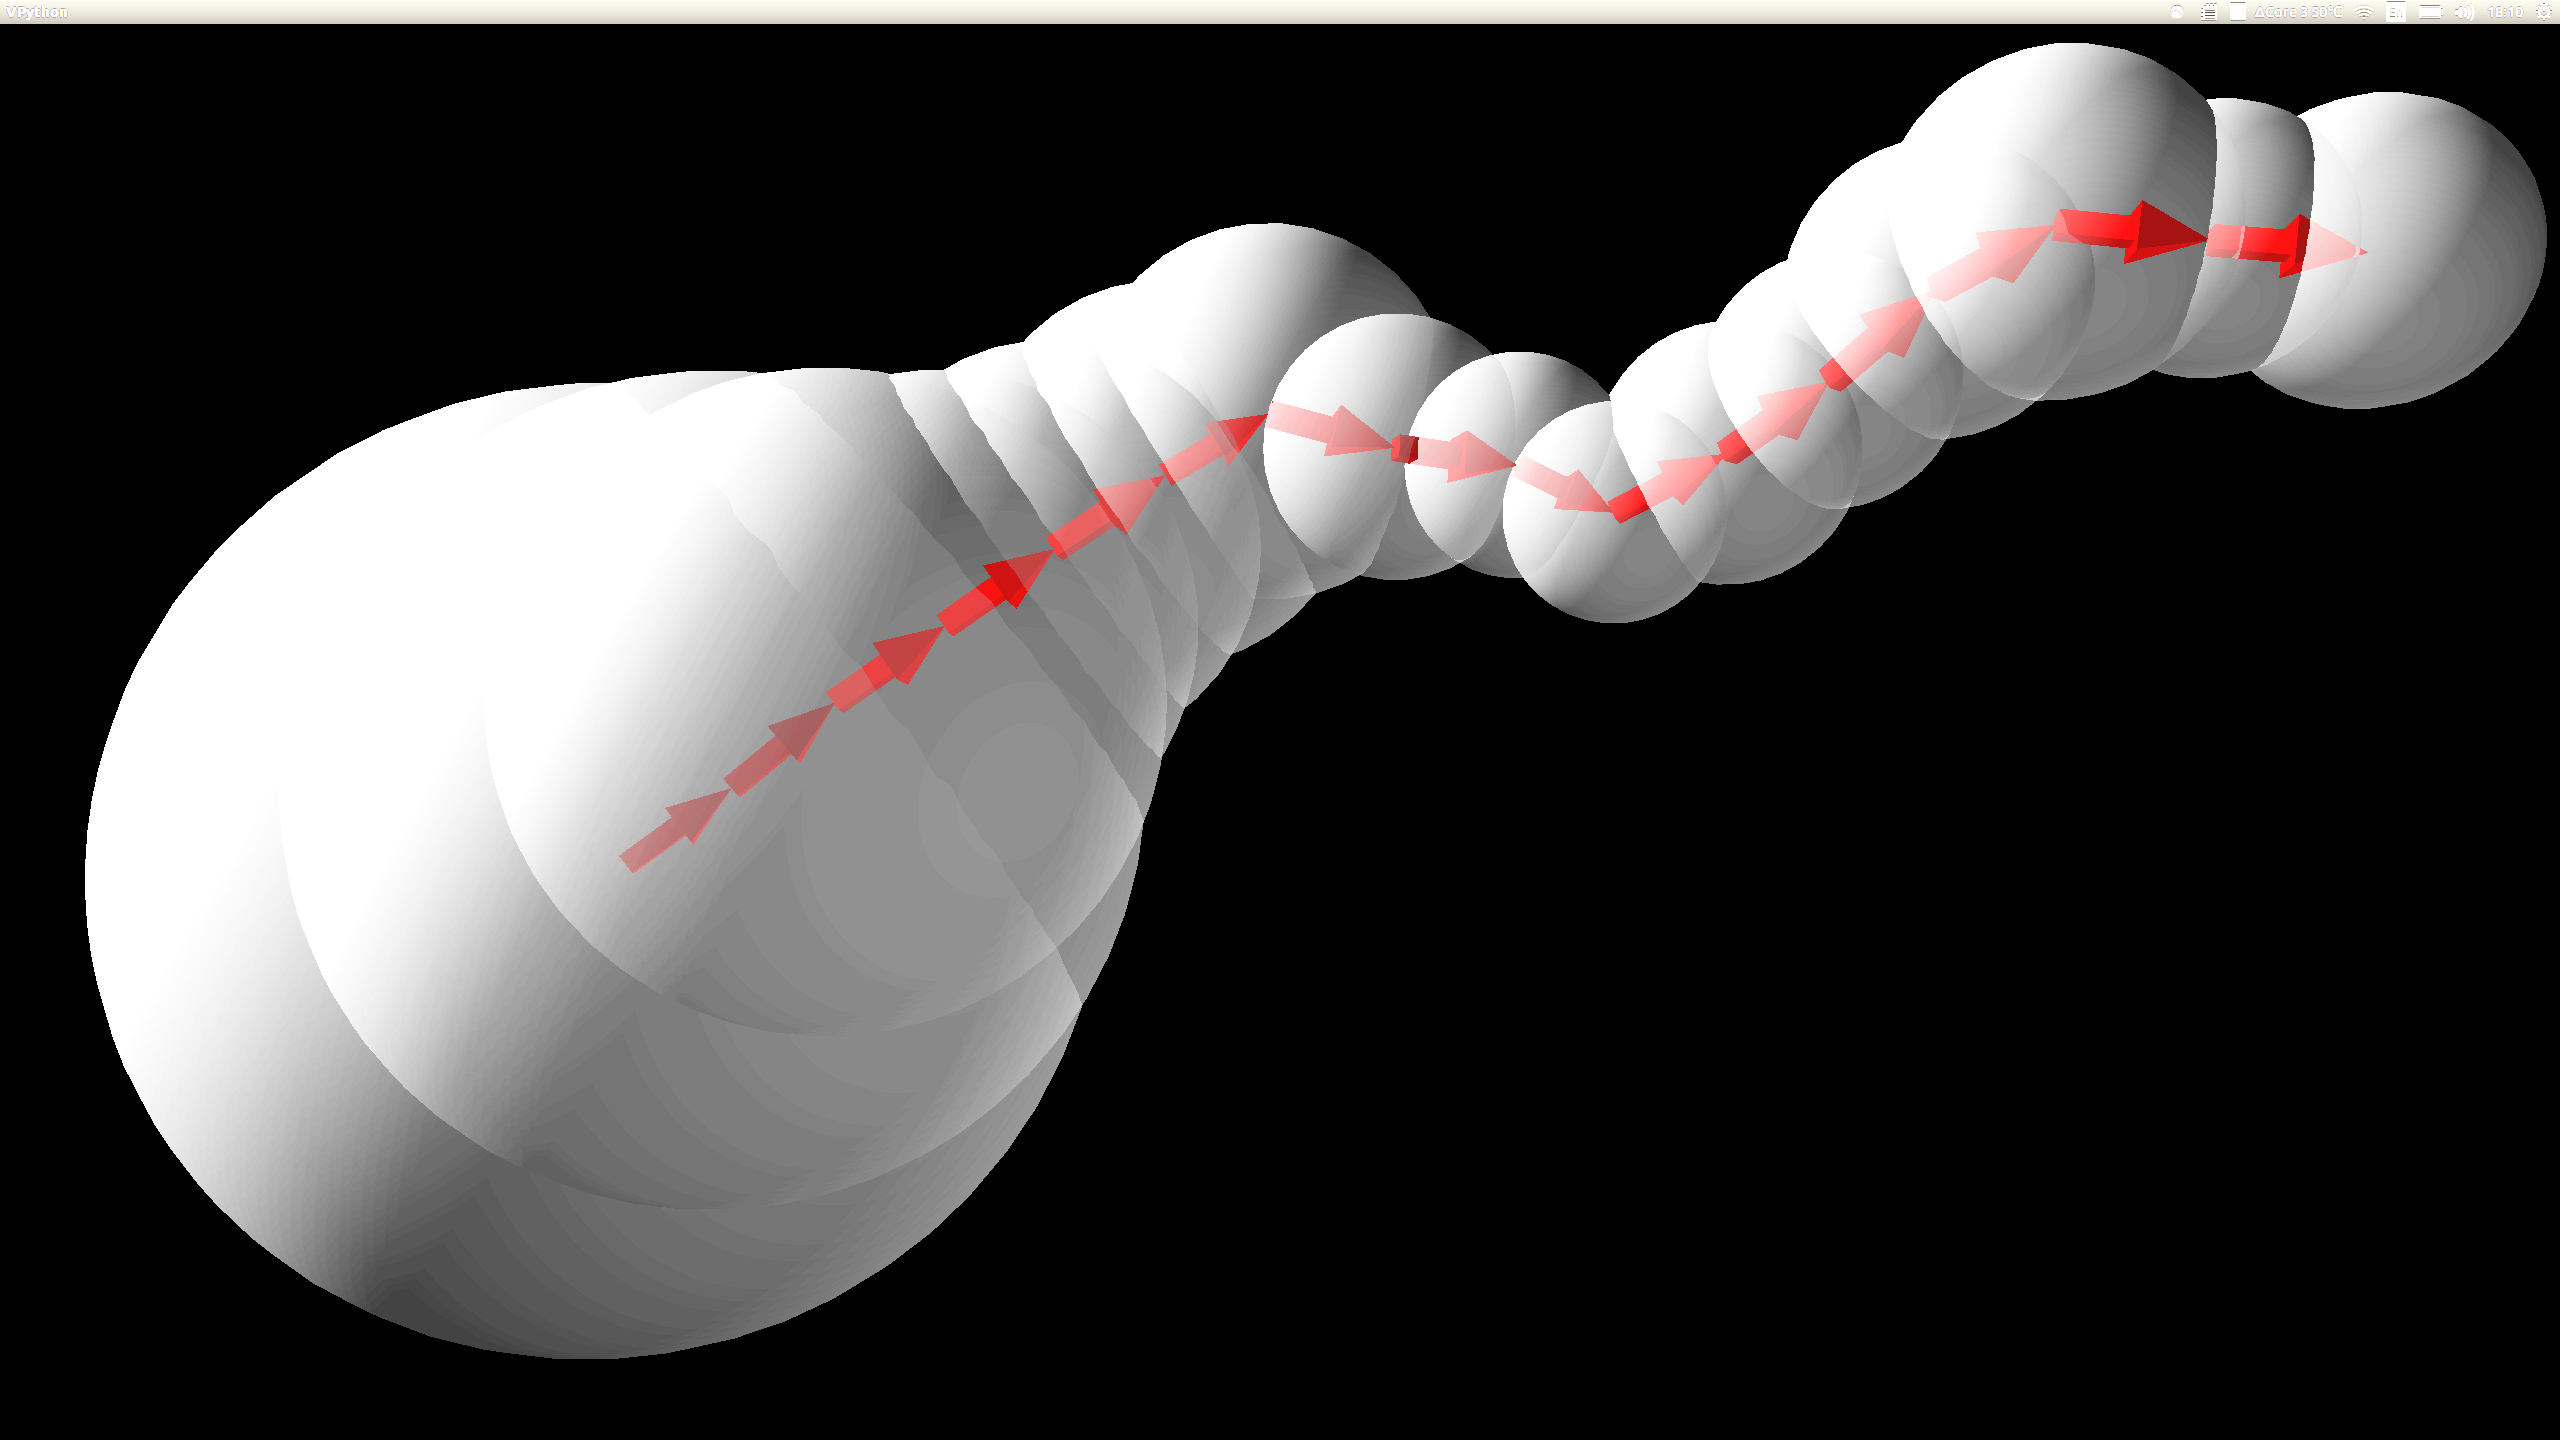
\includegraphics[width=100mm]{img/basic_tunnel.jpg}
	\caption{Sample of molecule tunnel}
  \centering
  \label{fig:basic_tunnel}
\end{figure}


Abychom mohli provádět docking ligandu, musíme nejprve takto definovaný tunel nařezat na jemné plátky - kruhy, na které pak v průběhu výpočtu budeme dokovat průběžné konformace ligandu. Popišme si nyní, jak by takové řezy měly vypadat.

\begin{defi}
Řezem tunelu $ \Tau $ rozumíme kruh v prostoru, který je určen uspořádanou trojicí $\theta = (A, u, r)$, kde $ A $ je střed, $ u \in \Rbb^3 $ je normálnový vektor a $ r > 0 $ je poloměr.
Pro tento kruh $ \theta $ musí platit, že $ \Tau \cap \theta $ je souvislá množina a navíc
$ \exists \delta > 0 $ tak, že $ \forall \varepsilon > 0,  \varepsilon < \delta $ je  $ (A, u, r + \varepsilon) \cap \Tau = \theta \cap \Tau $.
(Alternativně řečeno $\Tau \setminus \theta $ má dvě komponenty.)
\end{defi}

Uvedená definice prakticky říká, že řez tunel řeže jen na jednom místě (podmínka souvislosti). Druhá podmínka znamená, že řez je úplný, tedy že řezem skutečně rozdělíme tunel na dvě části.
Pro ilustraci, jak takové řezy mohou vypadat, přikládáme obrázek č. \ref{fig:tunnel_cuts}.
\begin{figure}[ht]
    \centering
    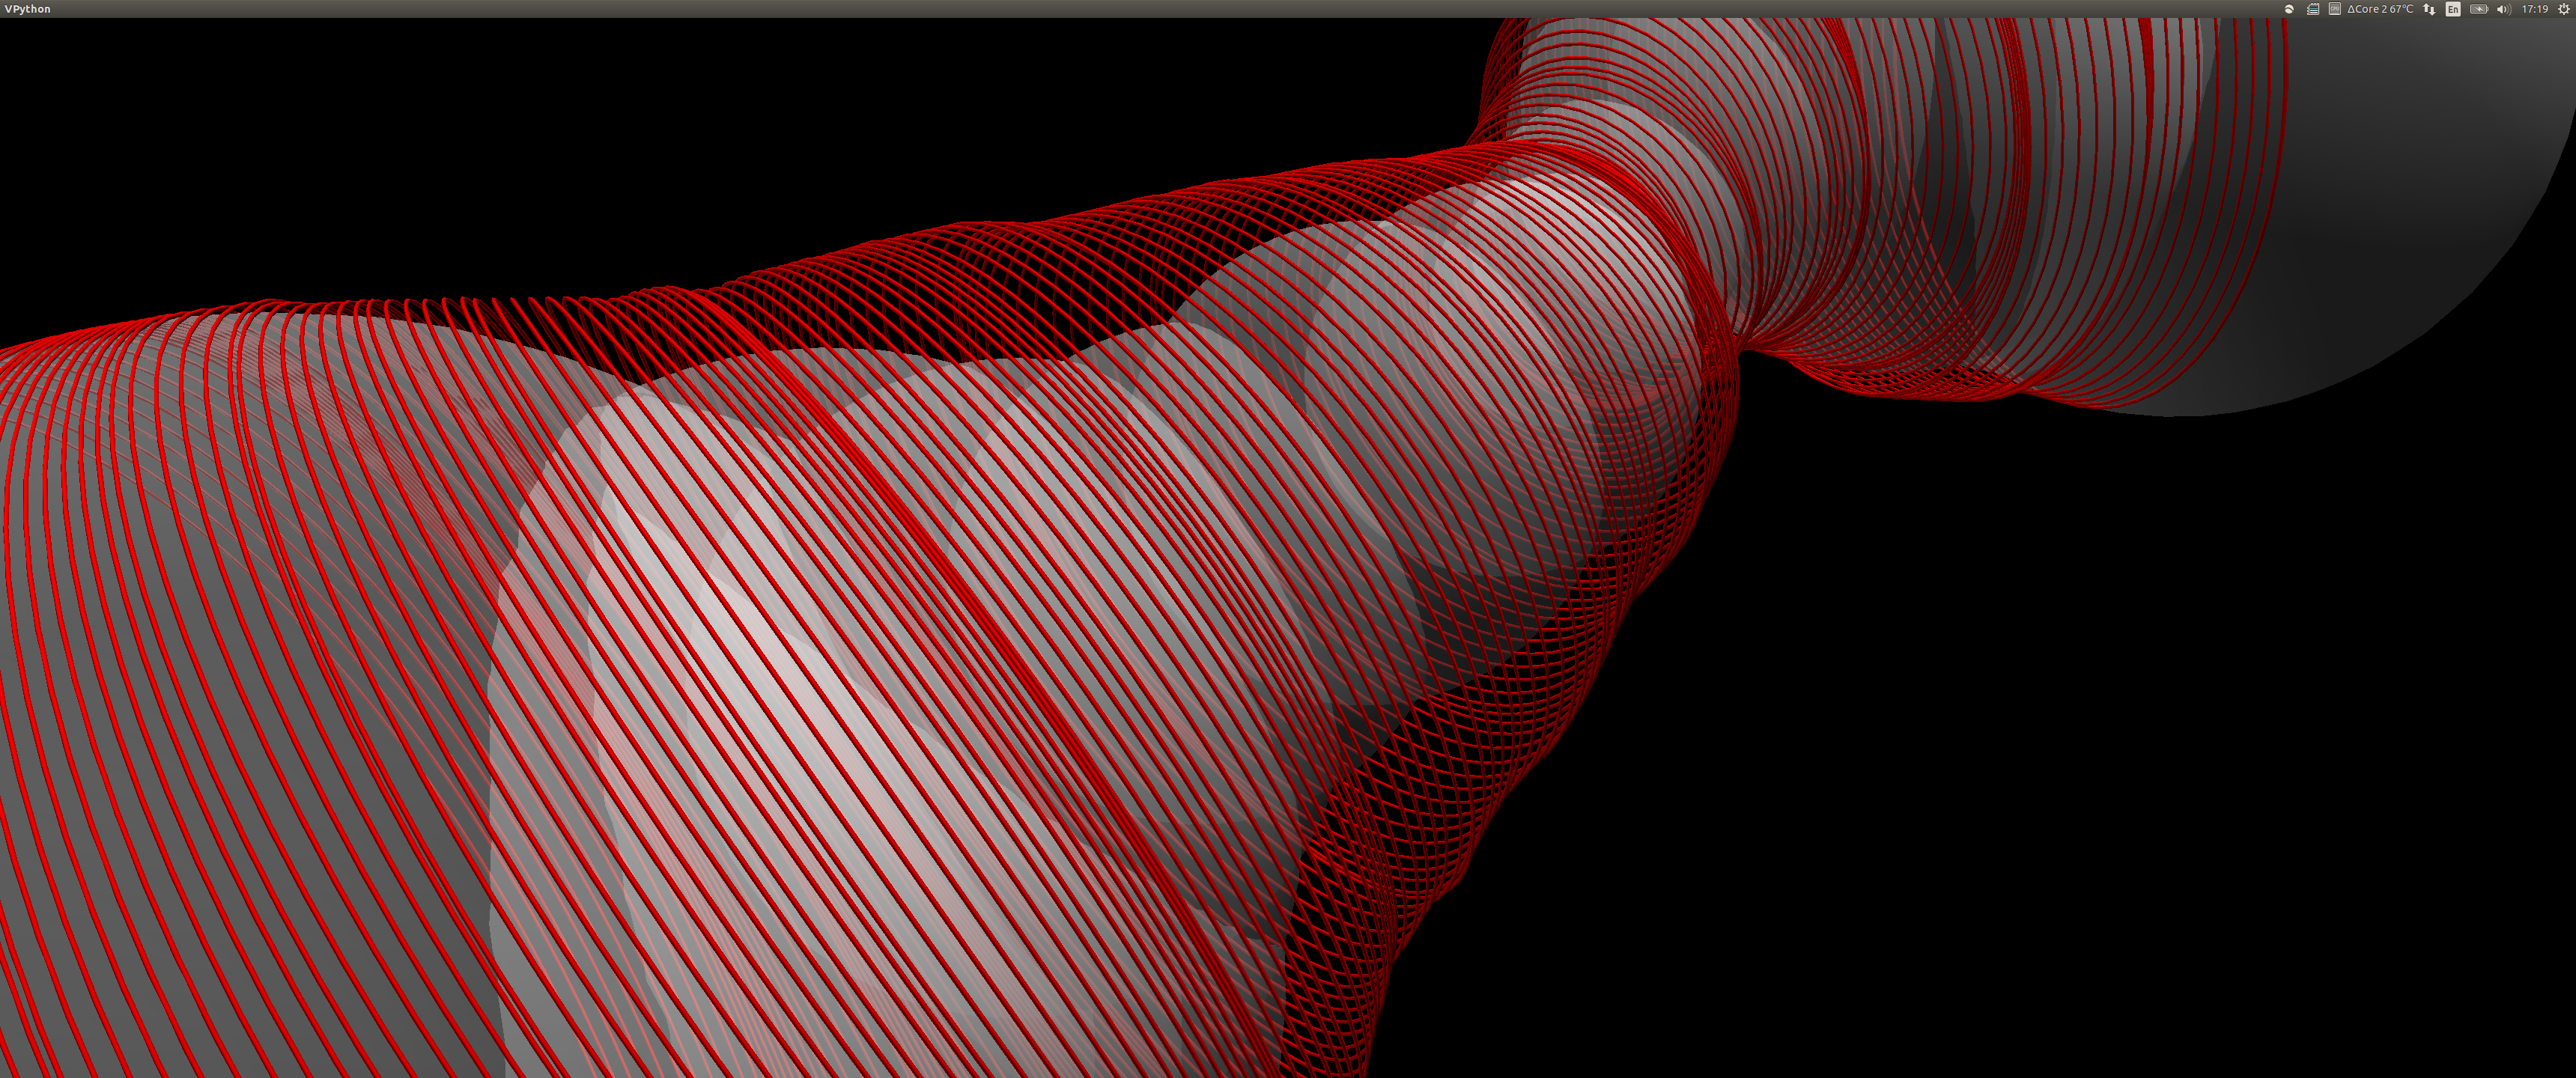
\includegraphics[width=\textwidth]{img/simple_cuts.png}
    \caption{Sample of molecule tunnel}
  \centering
  \label{fig:tunnel_cuts}
\end{figure}

S takto definovanými řezy můžeme začít uvažovat o tom, jak tunel nařezat jako celek.
Mějme $ \Theta = \{\theta_i\}_{i=0}^{k}$ posloupnost řezů tunelu $ \Tau $. Pro potřeby správného
dockingu bude nezbytné, aby platilo $ x, y \in \Theta \Rightarrow |x \cap y| \leq 1 $,
tedy každé dva řezy se dotýkají nejvýše v jednom bodě. Dále budeme chtít, aby po sobě
jdoucí řezy od sebe \textit{nebyly příliš daleko}. Vzdálenost budeme měřit pomocí funkce
$ \dst(x, y) $, kterou popisuje následující definice.

\begin{defi}
Mějme řezy $ x = (A, u, r_1), y = (B, v, r_2) \in \Theta $. Rozlišíme dvě situace
    \begin{enumerate}[label={(\arabic*)}]
        \item $ u = v $, pak $ \dst(x, y) = |B - A|$,
        \item v opačném případě $u, v$ určují rovinu $ \varrho = \langle u, v \rangle $.
        Kolmou projecí do roviny $ \varrho $ promítneme řezy $x $ resp. $y$, čímž získáme dvě úsečky
        určené vrcholy $X_1, X_2 $ resp $Y_1, Y_2 $. Vzdálenost pak definujeme jako
        $ \dst(x, y) = \min\{ \max\{|X_1 - Y_1|, |X_2 - Y_2|\}, \max\{|X_1 - Y_2|, |X_2 - Y_1|\}\}$.
    \end{enumerate}
\end{defi}

\end{document}
